\documentclass[10pt,conference,compsocconf]{IEEEtran}

%\usepackage{times}
%\usepackage{balance}
\usepackage{url}
\usepackage{graphicx}	% For figure environment
%\usepackage{subfig}
\usepackage{subcaption}
\usepackage{gensymb} % adds the \degree symbol

\begin{document}
\title{Road Extraction from Aerial Images using Denoising Autoencoders}

\author{
  Florian Chlan, Samuel Kessler, Yu-chen Tsai\\Group: CollaborativePilfering\\
  Department of Computer Science, ETH Zurich, Switzerland
}

\maketitle

\begin{abstract}

This article describes the pixelwise binary classification problem of detecting roads from aerial images. Two Convolutional Neural Networks were used as a baseline classifiers, with F1 scores of 0.77 and 0.86 respectively. An extension to the Convolutional Neural Network objective function using Median Frequency Class Balancing achieved an F1 score of 0.90. Extensions were made using a Denoising Autoencoder and Denoising Convolution Autoencoder to smooth out the outputs of the downstream Convolutional Neural Networks. The Denoising Convolutional Autoencoder produced an F1 score of 0.91.
  
\end{abstract}

\section{Introduction}

The problem of image segmentation has been boosted by the relatively recent advancements in Deep Learning. Image segmentation underpins tasks from the detection of cancerous tissues in medical images to disrupting the delivery market with autonomous drone deliveries. The work introduced in this article may be applied to any image segmentation problem.

The report outlines a couple approaches to the image segmentation task of extracting roads from aerial images. The baseline Convolutional Neural Network (CNN) models produced good results (see \ref{Baseline1} and \ref{Baseline2} for implementation details and \ref{Results} for details on performance). The CNN models produced noisy outputs to the image segmentation problem, subsequently the focus was to denoise these outputs.

The focus of the work demonstrated in this article is on the denoising of the CNN output. A Denoising Autoencoder (DAE) was employed to learn a low dimensional representation the road network to segment the images (see \ref{DAE} for the implementation details). 

The DAE was naturally extended to a Convolutional Denoising Autoencoder (CDAE). The CDAE was shown to denoise the outputs of the CNN and improve the performance of the image segmentation (see section \ref{CDAE} for implementation details and \ref{Results} for the results).

\section{Data}

The training data set contains 100 colour images of 400x400x3 resolution while the test data set was comprised of 50 colour images of 608x608x3 resolution (an example may be seen in figure \ref{fig:classbalancing}). Each pixel in the training images has a corresponding binary label indicating whether it is part of a road or not. Validation is performed via a holdout dataset on the Kaggle online platform.

\section{Models and Methods}
\label{MM}

\subsection{Baseline 1}
\label{Baseline1}

\subsubsection{Implementation}
The first baseline used 16x16x3 pixel patches as an input, where each patch is assigned to a single class. Approximately $\frac{3}{4}$ of the training patches are labelled as background and the remaining patches as road. Classes were balanced by throwing away excess data from the background class. The first baseline uses two convolutional layers with 5x5 filters and the feature maps expanding to 32 and 64 respectively. 2x2 Max-pooling is used with a stride of 2. Finally two fully connected layers are used to rein in the network, down to two nodes for the binary classification task. ReLU activation functions are used. Cross entropy loss with a softmax is optimized with stochastic gradient descent (SGD) and with an exponentially decreasing learning rate. The network weights are regularized with a penalization of $5\times10^{-4}$.

\subsection{Baseline 2}
\label{Baseline2}
\subsubsection{Implementation}
The second baseline used a CNN implemented by a previous group who worked on the same road extraction problem \cite{mato}. The second baseline utilizes a context of size 32x32 to predict a 8x8 patch lying at its centre. The use of a large context to discern road from roof or tree is the crux of the model. Images are downsized to half the original dimension size via interpolation for lower computational cost. Image boundaries were mirrored for predictions at the image's edge. Patches were extracted with a stride of 1 and the set of patches augmented with $90 \degree$ rotations.

The CNN architecture is deeper than that of the first baseline \ref{Baseline1}: using four convolutional layers with a first 5x5 filter then 3x3 filters for the remaining layers. The feature maps increase gradually to 64. Finally two fully-connected layers are used to funnel the network down to two nodes for the classification task. At each layer, ReLU activation functions and local response normalisation \cite{Krizhevsky2012} is applied. Cross entropy with softmax is used as the loss function. For further details see \cite{mato}.

\subsection{Median Frequency Class Balancing}
\label{classbalancing}
\subsubsection{Motivation}
The two baselines, (\ref{Baseline1} and \ref{Baseline2}) employed a rudimentary class balancing strategy, which resulted in about $\frac{2}{3}$ of the background patches being thrown away: $\frac{1}{2}$ of the overall training data. To ensure all precious training data is used in training, Median Frequency Class Balancing (MFCB) \cite{Eigen2016} \cite{DBLP:journals/corr/BadrinarayananK15} was employed. 
\subsubsection{Implementation}
MFCB weighted the two classes in the loss function according to the ratio of the median frequency of all classes and the respective class frequency. Hence the dominant background class will received a lower weight than the road class and importantly no training data required discarding.

The median frequency class balancing strategy was applied to the CNN from Baseline 2, see figure \ref{fig:classbalancing} for an example of the output.

\begin{figure}[h!]
%%\centering  % not needed as the subfigures are maximally separated

\begin{subfigure}{0.2\textwidth}
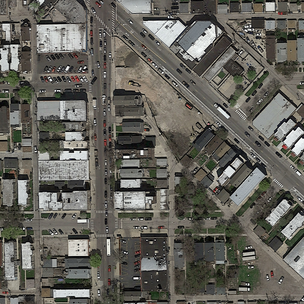
\includegraphics[width=\linewidth]{test_11.png}
\caption{Aerial image from test data set.}
\label{fig:test}
\end{subfigure}
\hspace*{\fill}
\begin{subfigure}{0.2\textwidth}
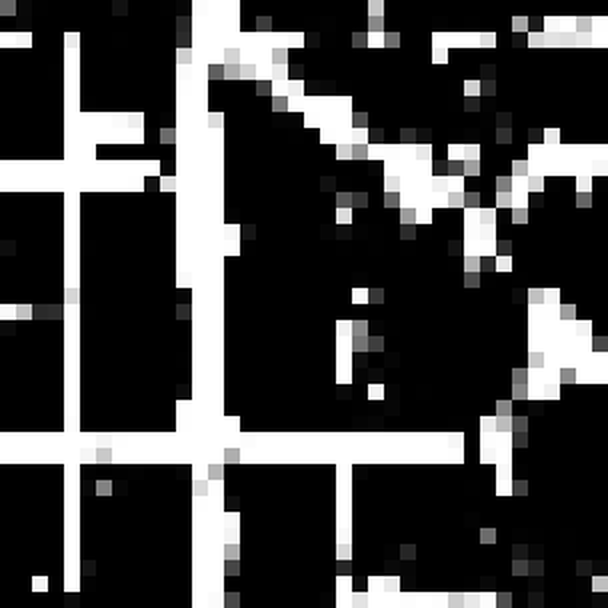
\includegraphics[width=\linewidth]{raw_test_11_pixels.png}
\caption{Output from a the CNN with MFCB}
\label{fig:MFCB}
\end{subfigure}

\caption{Prediction of the CNN with MFCB, the image on the left is a test image input and the grey scale image on the right is the predicted output.}
\label{fig:classbalancing}
\end{figure}

\subsection{Denoising Autoencoder}
\label{DAE}

\subsubsection{Motivation}

Qualitatively it was noticed that the output of the MFCB, figure \ref{fig:MFCB}, produces noisy results. Hence the need to a method able to denoise these images.

The road network of the aerial image is comprised mostly of straight lines. The road network exists in a low dimensional manifold; hence the use of an autoencoder to learn the low dimensional representation. Furthermore, by adding noise to the training input, the DAE is able to learn a mapping from the corrupted data to the uncorrupted true data manifold where the road network resides. In corrupting the input data, the corrupted examples are more likely to lie outside the manifold than uncorrupted examples, hence the autoencoder learns this mapping to the manifold \cite{VincentPASCALVINCENT2010}. 

\begin{figure}[!htb]
\minipage{0.15\textwidth}
  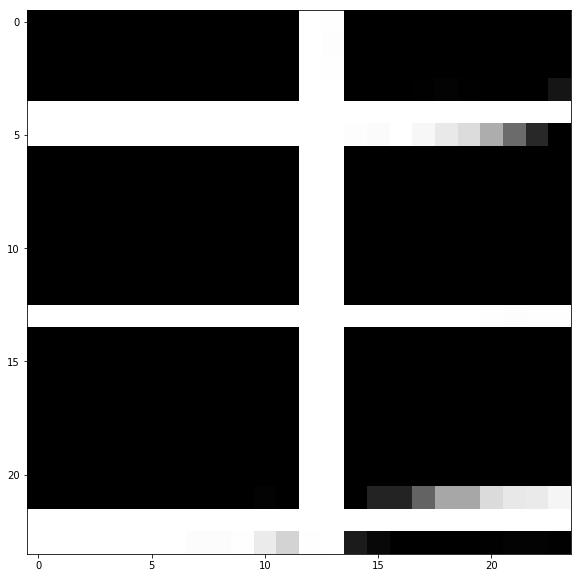
\includegraphics[width=\linewidth]{NoiseExamples_Uncorrupted.png}
  \caption{Uncorrupted image}\label{fig:nonoise}
\endminipage\hfill
\minipage{0.15\textwidth}
  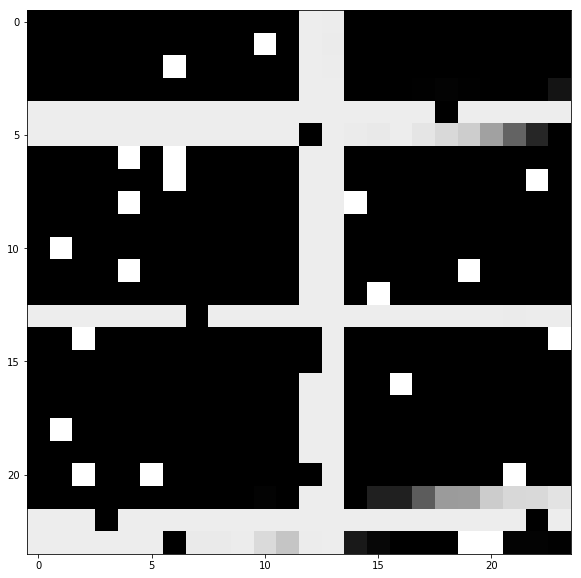
\includegraphics[width=\linewidth]{NoiseExamples_SaltNPepper.png}
  \caption{Salt and pepper noise}\label{fig:saltnpepper}
\endminipage\hfill
\minipage{0.15\textwidth}%
  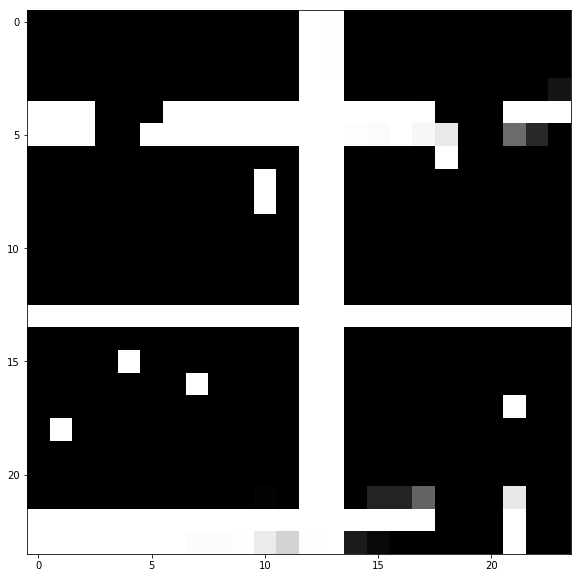
\includegraphics[width=\linewidth]{NoiseExamples_RandomNeighbourhood.png}
  \caption{Random neighbour noise}\label{fig:neighbour}
\endminipage
\end{figure}

\subsubsection{Corruption Processes}

A salt and pepper noise \cite{VincentPASCALVINCENT2010} was considered suitable for the corruption process: a fraction $\nu$ of the pixels of the input images are flipped to the minimum of maximum intensities.

The salt and pepper noise was not perfectly loyal to the noise observed in the output of the CNN. For example, the outputs of the CNN has clusters of pixels which are of one class which break up a road in two, in addition to isolated noisy pixels. With this a priori knowledge, a new corruption method "random neighbourhood" was implemented. Similarly to salt and pepper noise, a random fraction $\nu$ of the pixels are chosen and flipped. Furthermore, pixels in the immediate 8-neighbourhood are each flipped at random with a probability of 90\% if the centre pixel is flipped from road to background. If the centre pixel is flipped from background to road, each neighbouring pixel is flipped with a probability of only 2.5\% only. Figure \ref{fig:saltnpepper} and \ref{fig:neighbour} show examples of the two corruption methods. 

\begin{figure}[h!]
%%\centering  % not needed as the subfigures are maximally separated

\begin{subfigure}{0.2\textwidth}

\includegraphics[width=\linewidth]{raw_test_14_pixels.png}
\caption{Output of the CNN.}
\label{fig:DAE1}
\end{subfigure}
\hspace*{\fill}
\begin{subfigure}{0.2\textwidth}
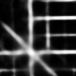
\includegraphics[width=\linewidth]{ae_test_14.png}
\caption{Output from a DAE.}
\label{fig:DAE2}
\end{subfigure}

\caption{Comparison of the output of the CNN with the output of the DAE. The DAE heavily smooths out input images: noise and irregular roads are smoothed away completely.}
\label{fig:DAE}
\end{figure}

\subsubsection{Implementation}

Images output by the CNN were downsampled such that a single pixel comprised a single class. Patches of size 24x24 pixels with stride of 1 pixel were extracted and rotated by $45\degree$, $90\degree$ and $135\degree$. The ground truth patches were corrupted with $\nu=7.5\%$ and used as training data, with the uncorrupted ground truth used as the DAE target. 2 hidden layers were used. Around 10 nodes at the bottleneck produced the best results. Increasing the number of hidden layers in the encoder and decoder from 2 up to 5 did not qualitatively improve the prediction images. Sigmoid activation functions were used and performed better than ReLUs. A mean squared error objective function is employed. An Adam optimizer with a learning rate of 0.005 was used. No dropout was used: a small amount of dropout was shown to heavily regularize the outputs; the DAE would ignore features of the input image and draw roads in places were the input image did not have any.

Stacking autoencoders as described in \cite{VincentPASCALVINCENT2010} was also tried, but from observation were seen to heavily generalize the inputs images.

An example of the output of the DAE can be seen in figure \ref{fig:DAE}. The DAE is able to learn the manifold of the road network, however at the cost of small irregular road features which are ignored.

\subsection{Denoising Convolutional Autoencoder}
\label{CDAE}

\subsubsection{Motivation}

The DAE is able to learn the general features of the road network, but ignores more local features, such as small roads and dead-ends. For a more local denoising a DCAE is employed. 

\subsubsection{Implementation}

The setup is identical to the DAE, see section \ref{DAE} for further details, however the architecture of the network as changed. The encoding uses 2 convolutional encoding layers with filters sizes 5x5 and then 3x3 and feature maps of increased to 16 and 32 respectively. Two deconvolutional layers with transposed filter size 5x5 and the number of features maps reduced to the 1. ReLU activation functions were utilized and a mean squared error loss function used as an objective. The optimization was performed with the Adam optimization algorithm with a constant learning rate of 0.005. Salt and pepper corruption of $\nu=7.5\%$ is used. The "random neighbourhood" corruption was also employed with a $\nu=5\%$ with no change in the predictive performance of the DCAE.

Increasing the number of layers did not produce significant improvements to the results, and adding skip connections, see \cite{DBLP:journals/corr/MaoSY16a} for further details, did not improve the performance of the deep CDAE networks.

\begin{figure}[h!]
\begin{subfigure}{0.2\textwidth}

\includegraphics[width=\linewidth]{cnn_41.png}
\caption{Output of the CNN.}
\label{fig:DAE1}
\end{subfigure}
\hspace*{\fill}
\begin{subfigure}{0.2\textwidth}

\includegraphics[width=\linewidth]{cae_41.png}
\caption{Output from a CDAE.}
\label{fig:DAE2}
\end{subfigure}

\caption{Comparison of the output of the MFCB CNN with the output of the CDAE. The CDAE output has been binarized with a threshold of 0.2, above which pixels are classified road.}
\label{fig:CDAE}
\end{figure}

Figure \ref{fig:CDAE} visualizes an prediction output from the DCAE. The roads have been smoothed out and in some instances joined up where there was a gap.

\section{Results and Discussion}
\label{Results}

The classification performance of the different models explored in section \ref{MM} are summarized in table \ref{table:1}. 

\begin{table}[h!]
\centering
\begin{tabular}{|l|l|}
\hline
Model & F1 Score \\ [0.5ex]
\hline
Baseline 1 & 0.778  \\
\hline
Baseline 2 & 0.856  \\
\hline
Baseline 2 + MFCB & 0.907  \\
\hline
Baseline 2 + MFCB + DCAE & 0.914 \\
\hline
\end{tabular}
\caption{Results: Kaggle F1 scores for stated models.}
\label{table:1}
\end{table}

The class balancing (described in section \ref{classbalancing}) boosted the predictive performance significantly. The likely cause of this was due to the limited amount of training data for both baseline CNNs, simply throwing out training data seriously limited the performance of the classifier. For small training datasets like the dataset used in this study the MFCB method could be highly beneficial.

Despite the interesting results from the DAE, qualitatively the predictive performance of our end-to-end method would decrease. The best results from \cite{VincentPASCALVINCENT2010} came from using a noisy and rotated versions of the MNIST dataset. This dataset has smaller diversity than that of the road network dataset used here and might help explain the inability the replicate the performance cited. 

Qualitatively, the CDAE was able to smooth out the abnormalities in the output of the MFCB CNN: joining up roads which had been corrupted and smoothing them. The score of 0.91 on the hold-out set on Kaggle demonstrates a modest increase in the predictive performance of the method. The CDAE demonstrates that in image segmentation tasks where the output is noisy, a CDAE could be a good idea to denoise the segmented images.

\section{Summary}

The novel contributions demonstrated above are the introduction of the MCFB and DCAE methods to the problem of image segmentation in aerial images to extract roads. The MCFB was shown to significantly boost the predictive power of the CNN classifier and the DCAE was shown to the reduce the noise from the outputs of the CNN. Together these are able to improve the predictive performance of this prediction problem with respect to both baselines.\\

\bibliographystyle{IEEEtran}
\bibliography{cil_report}
\end{document}
